\chapter{Simulado 4}

\num{1} Um jogo consiste em uma pessoa sortear um número e, depois de ver
que número é esse, pensar por alguns instantes e dizer em qual potinho
deve ser colocado cada algarismo do número.

\begin{figure}[htpb!]
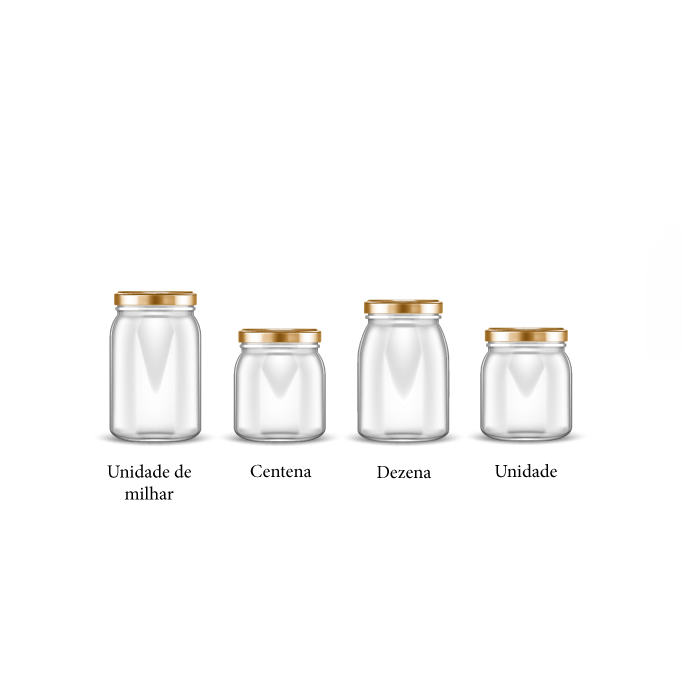
\includegraphics[width=\textwidth]{../ilustracoes/MAT5/SAEB_5ANO_MAT_figura123.png}
\end{figure}

O número que acabou de ser sorteado foi 3.756. Que algarismo será
colocado no potinho com rótulo centenas?

\begin{minipage}{.5\textwidth}
\begin{escolha}
\item
  7
\item
  6
\item
  5
\item
  3
\end{escolha}
\end{minipage}
\sidetext{SAEB: Identificar a ordem ocupada por um algarismo ou seu
valor posicional (ou valor relativo) em um número natural de até 6
ordens.

BNCC: EF05MA01 - Ler, escrever e ordenar números naturais até a ordem das 
centenas de milhar com compreensão das principais características do 
sistema de numeração decimal. 
EF05MA10 - Concluir, por meio de investigações, que a relação de 
igualdade existente entre dois membros permanece ao adicionar, subtrair, 
multiplicar ou dividir cada um desses membros por um mesmo número, para 
construir a noção de equivalência.
EF05MA11 - Resolver e elaborar problemas cuja conversão em sentença 
matemática seja uma igualdade com uma operação em que um dos termos é 
desconhecido.

a) Correta. No número 3.756, o algarismo que ocupa o valor posicional
de centena é o 7.
b) Incorreta. No número 3.756, o algarismo que ocupa o valor posicional
de centenas é o 7. 6 ocupa o valor da unidade. 
c) Incorreta. No número 3.756, o algarismo que ocupa o valor posicional
de centenas é o 7. 5 ocupa o valor da dezena.
d) Incorreta. No número 3.756, o algarismo que ocupa o valor posicional
de centenas é o 7. 3 ocupa o valor do milhar.}

\num{2} Jorge foi passar férias no sítio pertencente a sua família.
Chegando lá, correu até a horta e colheu 10 dezenas de pés de rúcula, 1
centena de espigas de milho, 5 dezenas de tomate, 2 unidades de cebola e
3 pepinos. Qual o total de produtos colhidos por Jorge?

\begin{minipage}{.5\textwidth}
\begin{escolha}
\item
  21
\item
  255
\item
  405
\item
  675
\end{escolha}
\end{minipage}
\sidetext{SAEB: Compor ou decompor números naturais de até 6 ordens na
forma aditiva, ou em suas ordens, ou em adições e multiplicações.

BNCC: EF05MA01 - Ler, escrever e ordenar números naturais até a ordem das 
centenas de milhar com compreensão das principais características do 
sistema de numeração decimal. 
EF05MA10 - Concluir, por meio de investigações, que a relação de 
igualdade existente entre dois membros permanece ao adicionar, subtrair, 
multiplicar ou dividir cada um desses membros por um mesmo número, para 
construir a noção de equivalência.
EF05MA11 - Resolver e elaborar problemas cuja conversão em sentença 
matemática seja uma igualdade com uma operação em que um dos termos é 
desconhecido.

a) Incorreta. Jorge colheu 255 produtos. 
b) Correta. 10 dezenas de pés de rúcula = 10 X 10 = 100 produtos.
1 centena de espigas de milho = 100 produtos. 5 dezenas de tomate
= 50 produtos. 2 cebolas e 3 pepinos = 5 produtos. Somando todos os
produtos teremos: 100 + 100 + 50 + 5 = 255.
c) Incorreta. Jorge colheu 255 produtos.
d) Incorreta. Jorge colheu 255 produtos.}

\num{3} Geraldo queria enviar um presente ao amigo José que mudou de
cidade. Ele se lembrava do nome da rua para a qual o amigo havia se 
mudado, mas não sabia qual o número da casa. Geraldo então enviou
uma mensagem ao amigo perguntando o número da casa e José respondeu da
seguinte maneira:

\begin{figure}[htpb!]
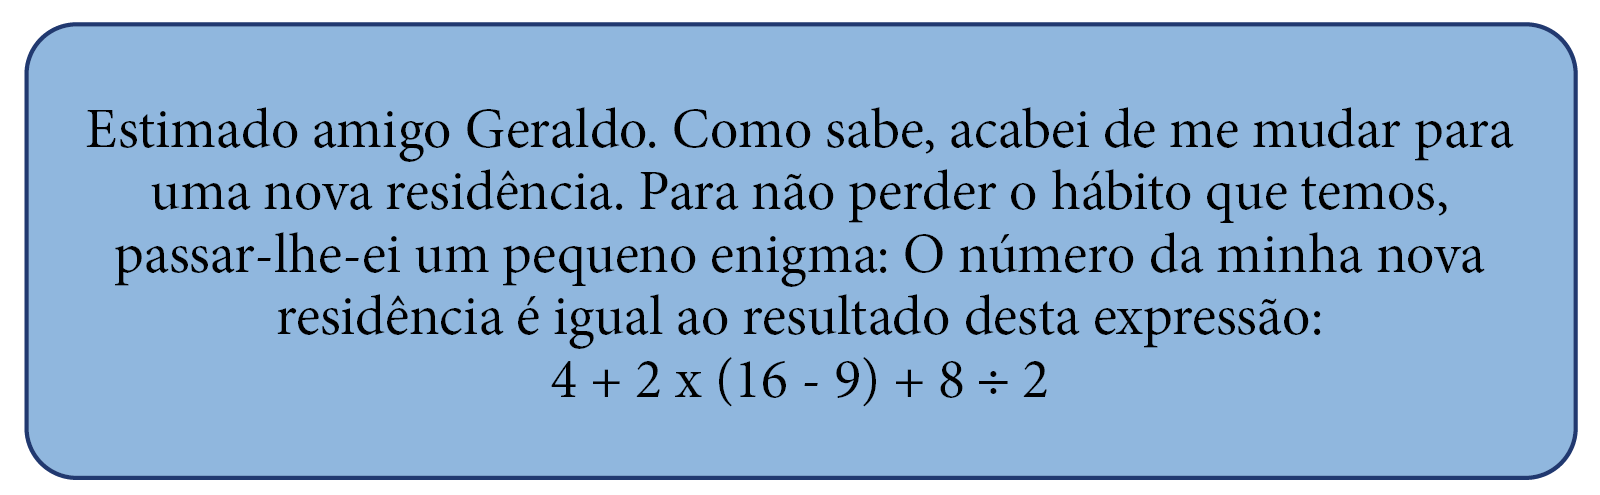
\includegraphics[width=\textwidth]{../ilustracoes/MAT5/SAEB_5ANO_MAT_figura124.png}
\end{figure}

%Acredito que haja um problema com este gabarito. A montagem da expressão numérica, sem distinção de parênteses e colchetes, permite chegar a mais de um resultado. Prefiro deixar essa avaliação para os leitores críticos. Provavelmente eles farão vários reparos, inclusive em páginas anteriores. (Rogério, 5/4/23, 9h07)

Qual o número da casa de José?

\begin{minipage}{.5\textwidth}
\begin{escolha}
\item
  13
\item
  20
\item
  22
\item
  28
\end{escolha}
\end{minipage}
\sidetext{SAEB: Resolver problemas de adição ou de subtração,
envolvendo números naturais de até 6 ordens, com os significados de
juntar, acrescentar, separar, retirar, comparar ou completar.

Resolver problemas de multiplicação ou de divisão, envolvendo números
naturais de até 6 ordens, com os significados de formação de grupos
iguais (incluindo repartição equitativa e medida), proporcionalidade ou
disposição retangular.

BNCC: EF05MA01 - Ler, escrever e ordenar números naturais até a ordem das 
centenas de milhar com compreensão das principais características do 
sistema de numeração decimal. 
EF05MA10 - Concluir, por meio de investigações, que a relação de 
igualdade existente entre dois membros permanece ao adicionar, subtrair, 
multiplicar ou dividir cada um desses membros por um mesmo número, para 
construir a noção de equivalência.
EF05MA11 - Resolver e elaborar problemas cuja conversão em sentença 
matemática seja uma igualdade com uma operação em que um dos termos é 
desconhecido.

a) Incorreta.
b) Incorreta.
c) Resposta: C. 4 + 2 x 7 + 8 / 2 = 4 + 14 + 4 = 22.
d) Incorreta.}

\num{4} Arnaldo esqueceu um dos números que fazem parte da senha do cofre
que tem em casa. Ele lembra que a senha era composta por 6
números e que os números da senha formam a seguinte sequência (2, 102,
202, \_\_A\_\_, 402, 502).

Através da análise da sequência podemos afirmar que o número A, o qual
ele esqueceu é:

\begin{minipage}{.5\textwidth}
\begin{escolha}
\item
  O dobro de 150
\item
  O antecessor de 303
\item
  O sucessor de 251
\item
  Metade de 500
\end{escolha}
\end{minipage}
\sidetext{SAEB: Inferir os elementos ausentes em uma sequência de
números naturais ordenados, objetos ou figuras.

a) Incorreta. O número que falta na sequência é 302.
b) Correta. O número que está faltando na sequência é 302 (antecessor 
de 303), pois, na sequência, somam-se 100 unidades ao número seguinte: 
2, 102, 202, 302, 402 e 502.
c) Incorreta. O número que falta na sequência é 302.
d) Incorreta. O número que falta na sequência é 302.}

\num{5} Considerando que todos os objetos abaixo estão cheios de água,
qual deles pode conter exatamente 3 litros de água?

\begin{figure}[htpb!]
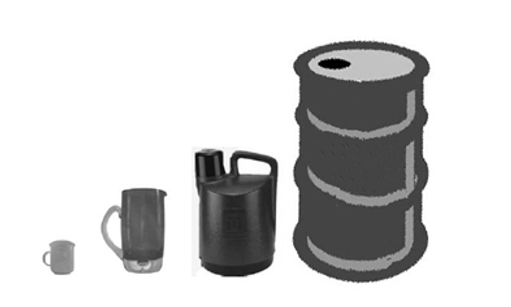
\includegraphics[width=.5\textwidth]{./imgs/mat22.png}
\end{figure}

%Pessoalmente julgo esta questão bastante ruim, baseada apenas no senso-comum, sem qualquer fundamento além dele. Tudo é discutível nesta questão, tudo depende da subjetividade. (Rogério, 5/4/23, 9h13)

\begin{minipage}{.5\textwidth}
\begin{escolha}
\item
  A caneca
\item
  A jarra
\item
  O garrafão
\item
  O tambor
\end{escolha}
\end{minipage}
\sidetext{SAEB: Estimar/inferir medida de comprimento, capacidade ou
massa de objetos, utilizando unidades de medida convencionais ou não ou
medir comprimento, capacidade ou massa de objetos.

a) Incorreta. 
b) Incorreta.
c) Correta. Pela análise figura podemos estimar que o garrafão
será o recipiente que pode conter exetamente 3 litos de água.
d) Incorreta.}

\num{6} Observe as figuras representadas na malha quadriculada abaixo:

\begin{figure}[htpb!]
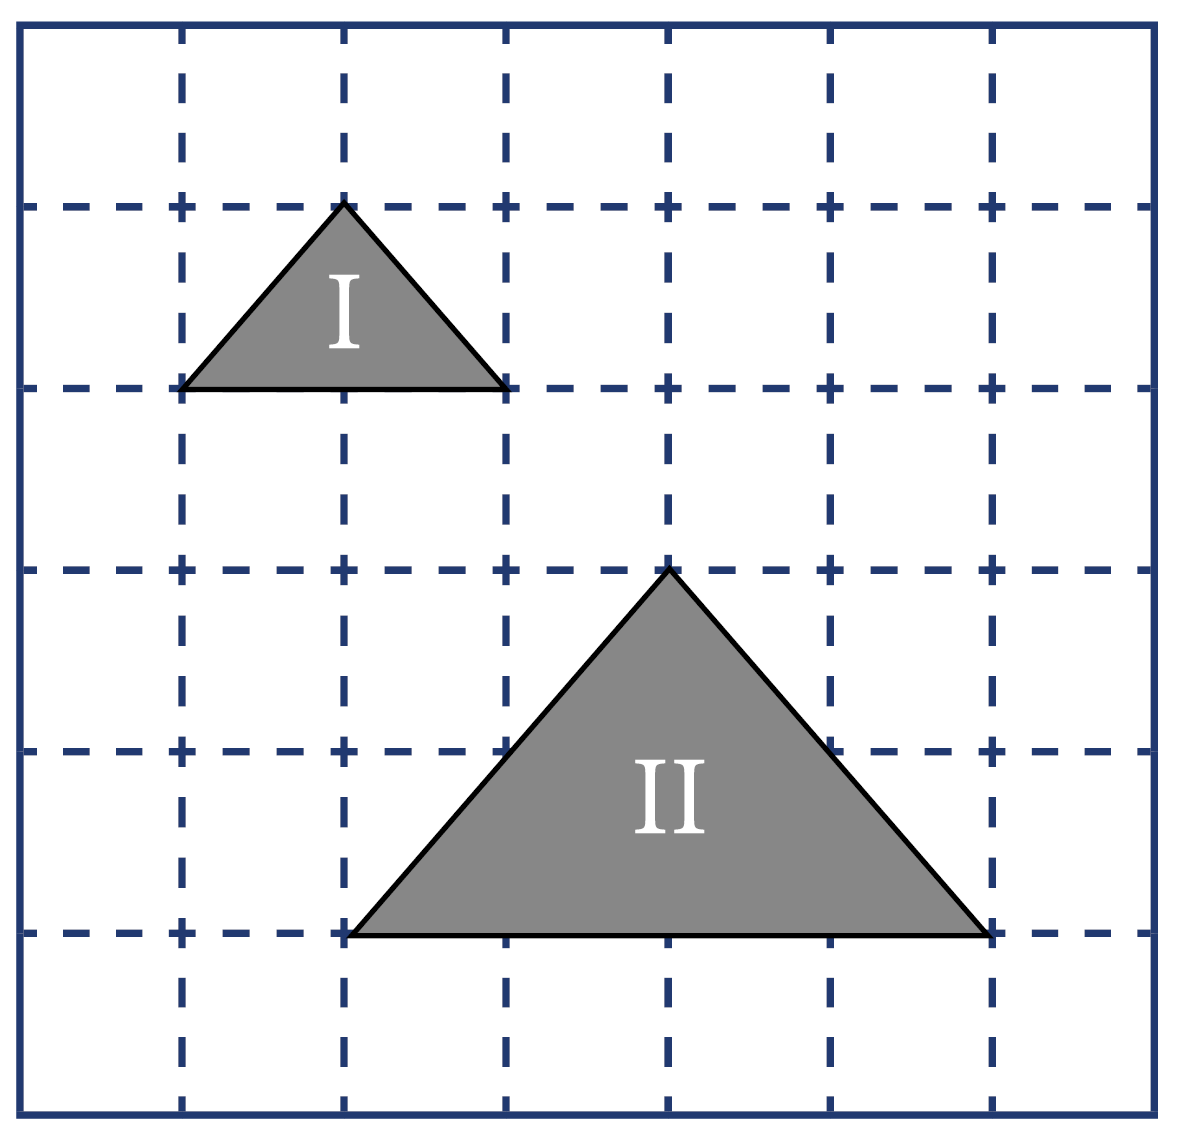
\includegraphics[width=\textwidth]{../ilustracoes/MAT5/SAEB_5ANO_MAT_figura125.png}
\end{figure}

Sabe-se que a figura II é um ampliação da figura I. O perímetro da
figura II, em relação ao perímetro da figura I, ficou:

\begin{minipage}{.5\textwidth}
\begin{escolha}
\item
  Reduzido à metade
\item
  Inalterado
\item
  Duplicado
\item
  Quadruplicado
\end{escolha}
\end{minipage}
\sidetext{SAEB: Medir ou comparar perímetro ou área de figuras planas
desenhadas em malha quadriculada.

a) Incorreta. O perímetro foi duplicado.
b) Incorreta. O perímetro foi duplicado.
c) Correta. Observando as figuras, percebe-se que a base do triângulo foi
duplicada (ela tinha dois quadradinhos na Figura I e tem quatro na Figura 
II), de modo que o perímetro também será duplicado.
d) Incorreta. O perímetro foi duplicado.}

\num{7} Rafael foi a uma papelaria e comprou um livro por R\$ 35,00 e uma
caneta por R\$ 3,00. Das alternativas abaixo, qual pode representar as
cédulas e moedas que Rafael utilizou para pagar, sabendo-se que não terá
troco?

\begin{minipage}{.5\textwidth}
\begin{escolha}
\item
  1 cédula de 10 reais, 5 cédulas de 5 reais e 3 moedas de 1 real.
\item
  1 cédula de 10 reais, 4 cédulas de 5 reais e 3 moedas de 1 real.
\item
  2 cédulas de 10 reais, 1 cédulas de 5 reais e 3 moedas de 1 real.
\item
  2 cédulas de 10 reais, 2 cédulas de 5 reais e 2 moedas de 1 real.
\end{escolha}
\end{minipage}
\sidetext{SAEB: Resolver problemas que envolvam moedas e/ou cédulas do
sistema monetário brasileiro.

a) Correta. 1 cédula de R\$ 10,00 será somado aos R\$ 25,00 das outras 
cinco cédulas e aos R\$ 3,00 das moedas. R\$ 10,00 + R\$ 25,00 + R\$ 3,00
= R\$ 38,00. 
b) Incorreta. O valor gasto por Rafael é R\$ 38,00, e o total proposto nesta alternativa é de R\$ 23,00.
c) Incorreta. O valor gasto por Rafael é R\$ 38,00, e o total proposto nesta alternativa é de R\$ 28,00.
d) Incorreta. O valor gasto por Rafael é R\$ 38,00, e o total proposto nesta alternativa é de R\$ 32,00.}

\num{8} Alana resolveu trocar todas as moedas que estavam em seu cofrinho
por uma única cédula. Ela tinha no cofrinho 10 moedas de 5 centavos, 5
moedas de 50 centavos, 70 moedas de 10 centavos.

Marque a alternativa que trás a nota correta que substituiu em valor
todas as moedas que Alana tinha em seu cofrinho:

\begin{figure}[htpb!]
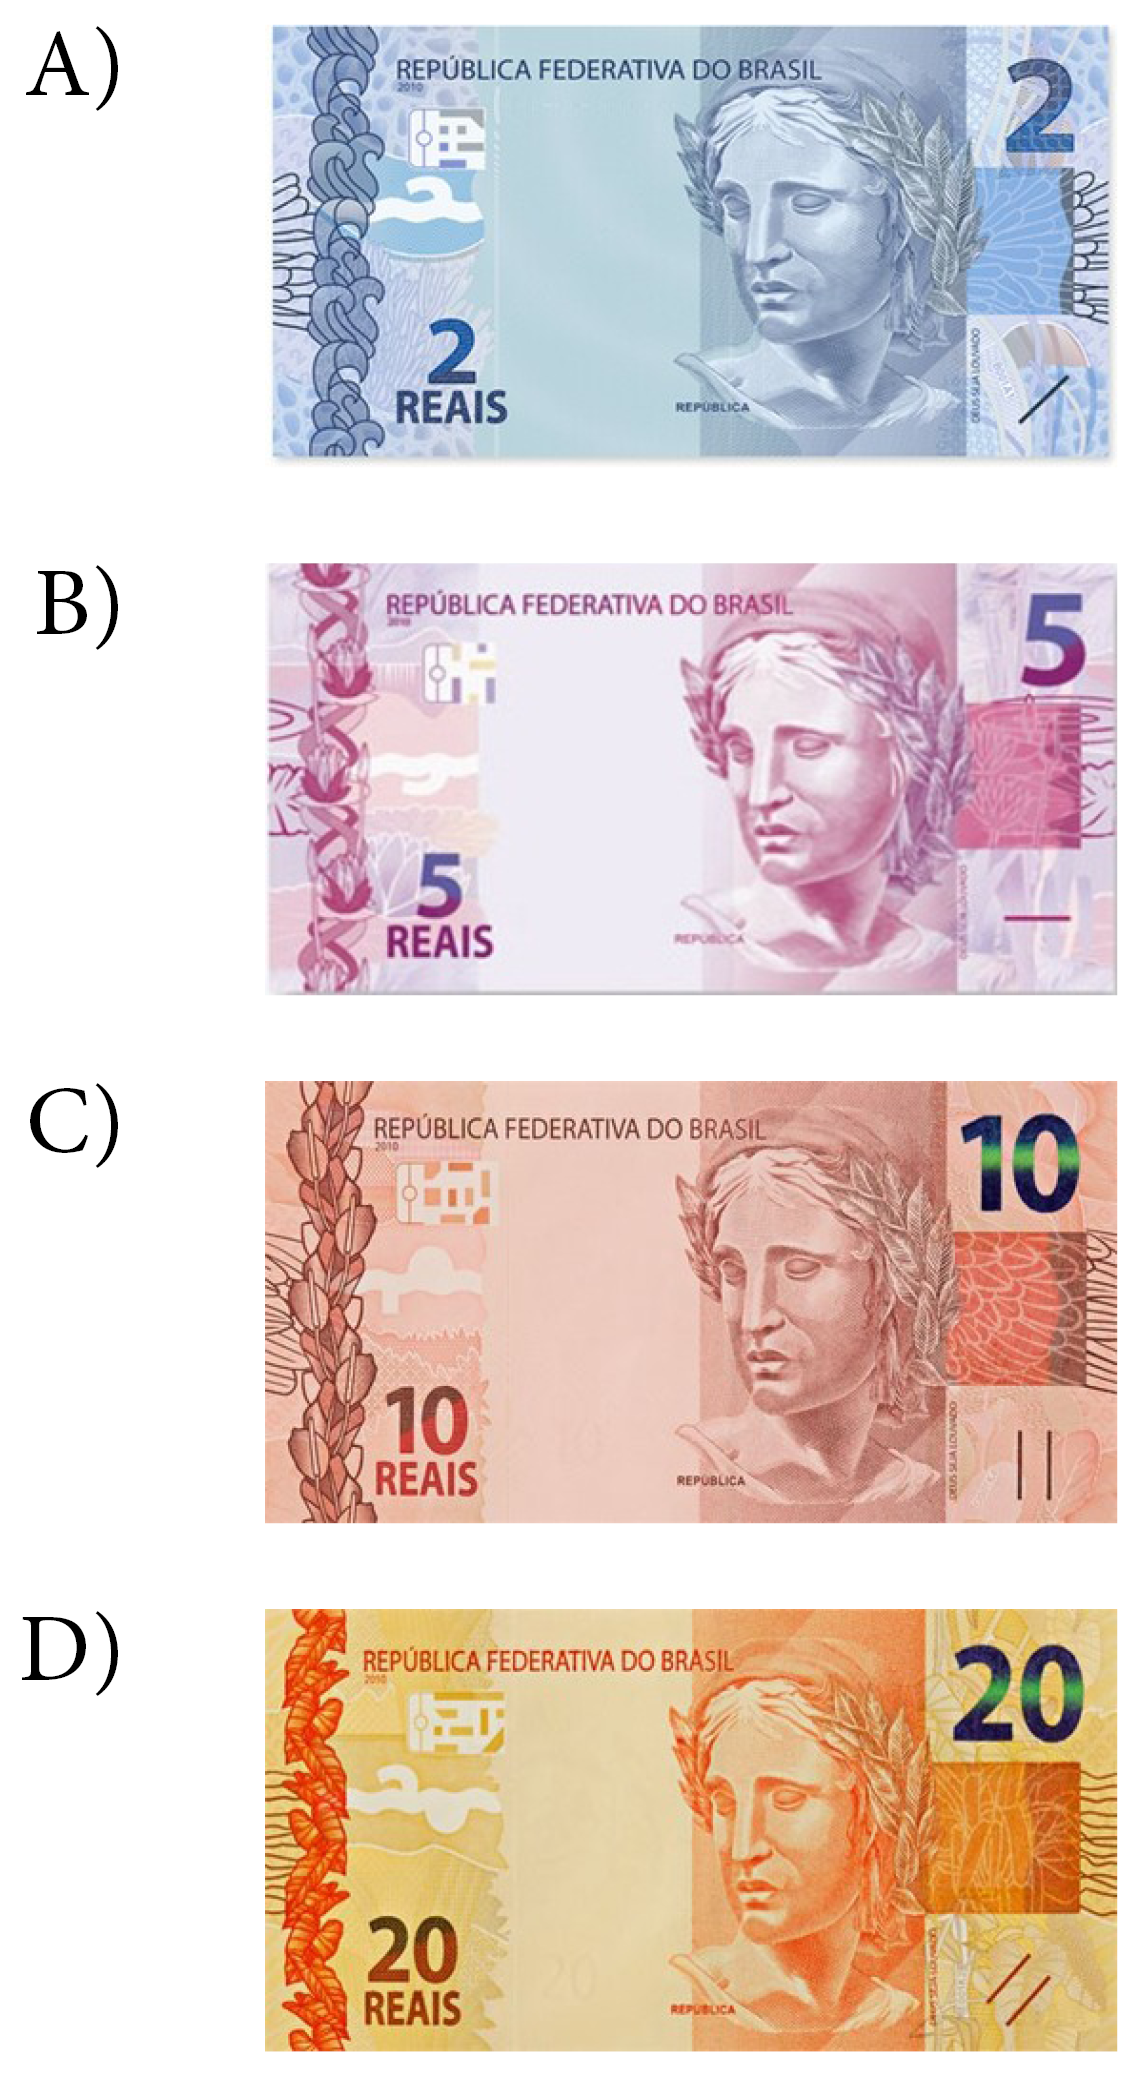
\includegraphics[width=\textwidth]{../ilustracoes/MAT5/SAEB_5ANO_MAT_figura126.png}
\end{figure}

\sidetext{SAEB: Relacionar valores de moedas e/ou cédulas do sistema
monetário brasileiro, com base nas imagens desses objetos.

a) Incorreta. O total no cofrinho de Alana é de R\$ 10,00.
b) Incorreta. O total no cofrinho de Alana é de R\$ 10,00.
c) Correta. 10 x 0,05 + 5 x 0,50 + 70 x 0,10 = 0,50 + 2,50 + 7 = R\$ 10,00. Portanto, Alana tem R\$ 10,00 no cofrinho.
d) Incorreta. O total no cofrinho de Alana é de R\$ 10,00.}

\num{9} Dentre os números naturais distintos de 1 a 20, escolhe-se um ao
acaso. Qual a probabilidade de se escolher um número par?

\begin{minipage}{.5\textwidth}
\begin{escolha}
\item
  10\%
\item
  35\%
\item
  50\%
\item
  90\%
\end{escolha}
\end{minipage}
\sidetext{SAEB: Determinar a probabilidade de ocorrência de um
resultado em eventos aleatórios, quando todos os resultados possíveis
têm a mesma chance de ocorrer (equiprováveis).

BNCC: EF05MA22 - Apresentar todos os possíveis resultados de um experimento aleatório, estimando se esses resultados são igualmente prováveis ou não.
EF05MA23 - Determinar a probabilidade de ocorrência de um resultado em eventos aleatórios, quando todos os resultados possíveis têm a mesma chance de ocorrer (equiprováveis).

a) Incorreta. A probabilidade de escolha de um número par é de 50\%.
b) Incorreta. A probabilidade de escolha de um número par é de 50\%. 
c) Correta. No conjunto de números apresentados, a metade é par, 
de modo que a probabilidade de se escolher um número par é de 50\%.
d) Incorreta. A probabilidade de escolha de um número par é de 50\%.}

\num{10} Em uma compeção de saltos ornamentais, cada atleta tem direito
a 3 saltos e sua pontuação final é dada pela soma dos 3 saltos. Ganha a
prova quem fizer o maior número de pontos no total.

A tabela abaixo mostra as notas obtidas por 5 atletas, A, B, C, D e E,
nos seus respectivos saltos:

\begin{tabular}{l|c|c|c}
\hline
\textbf{Atleta} & \multicolumn{1}{l|}{\textbf{Pontuação do 1º salto}} & \multicolumn{1}{l|}{\textbf{Pontuação do 2º salto}} & \multicolumn{1}{l}{\textbf{Pontuação do 3º salto}} \\ \hline
\textbf{A} & 6 & 6 & 6 \\ \hline
\textbf{B} & 7 & 3 & 8 \\ \hline
\textbf{C} & 5 & 7 & 6 \\ \hline
\textbf{D} & 5 & 6 & 8 \\ \hline
\end{tabular}

Analisando as notas de cada um dos atletas, podemos dizer que o campeão
foi o atleta:

\begin{minipage}{.5\textwidth}
\begin{escolha}
\item
  A
\item
  B
\item
  C
\item
  D
\end{escolha}
\end{minipage}
\sidetext{SAEB: Argumentar ou analisar argumentações/conclusões com
base em dados apresentados em tabelas (simples ou de dupla entrada) ou
gráficos (barras simples ou agrupadas, colunas simples ou agrupadas,
pictóricos ou de linhas).

a) Incorreta. O atleta A teve um total de 18 pontos (6 + 6 + 6), um a menos do que o atleta D.
b) Incorreta. O atleta B teve um total de 18 pontos (7 + 3 + 8), um a menos do que o atleta D.
c) Incorreta. O atleta C teve um total de 18 pontos (5 + 7 + 6), um a menos do que o atleta D.
d) O atleta D é o vencedor, porque obteve 19 pontos (5 + 6 + 8) -- um a mais do que os outros três atletas.}

\num{11} Em uma prova de automobilismo, o piloto que estava em
primeiro lugar sofreu com falta de combustível e precisou abandonar a
prova quando já tinha completado 2/7 da prova de 77 voltas no total.
Pode-se dizer que ele abandonou a prova depois de ter percorrido:

\begin{minipage}{.5\textwidth}
\begin{escolha}
\item
  11 voltas
\item
  22 voltas
\item
  30 voltas
\item
  44 voltas
\end{escolha}
\end{minipage}
\sidetext{SAEB: Resolver problemas que envolvam fração como resultado
de uma divisão (quociente).

BNCC: EF05MA03 - Identificar e representar frações (menores e maiores que a unidade), associando-as ao resultado de uma divisão ou à ideia de parte de um todo, utilizando a reta numérica como recurso.

EF05MA04 - Identificar frações equivalentes.

EF05MA06 - Associar as representações 10\%, 25\%, 50\%, 75\% e 100\% respectivamente à décima parte, quarta parte, metade, três quartos e um inteiro, para calcular porcentagens, utilizando estratégias pessoais, cálculo mental e calculadora, em contextos de educação financeira, entre outros.

a) Incorreta. O piloto abandonou a prova depois de 22 voltas.
b) Correta. 2/7 x 77 = 22 voltas.
c) Incorreta. O piloto abandonou a prova depois de 22 voltas.
d) Incorreta. O piloto abandonou a prova depois de 22 voltas.}

\num{12} Em uma mapa, a distância de 2.000 km entre duas cidades foi
representada por 16 cm. Qual a razão entre o valor desenhado no
mapa e a distância real entre as cidades?

\begin{minipage}{.5\textwidth}
\begin{escolha}
\item
  125
\item
  1/250
\item
  1/125
\item
  250
\end{escolha}
\end{minipage}
\sidetext{SAEB: Resolver problemas que envolvam variação de
proporcionalidade direta entre duas grandezas.

BNCC: EF05MA12 - Resolver problemas que envolvam variação de proporcionalidade direta entre duas grandezas, para associar a quantidade de um produto ao valor a pagar, alterar as quantidades de ingredientes de receitas, ampliar ou reduzir escala em mapas, entre outros.

a) Incorreta. 16/2000 = 1/125.
b) Incorreta. 16/2000 = 1/125.
c) Correta. 16/2000 = 1/125.
d) Incorreta. 16/2000 = 1/125.}

\num{13} Quantos números formados por 2 algarismos podemos formar com os
algarismos 1; 2; 3; 4; 5; 6; 7; 8 e 9 de forma que nenhum algarismo seja
repetido?

\begin{minipage}{.5\textwidth}
\begin{escolha}
\item
  81
\item
  72
\item
  100
\item
  64
\end{escolha}
\end{minipage}
\sidetext{SAEB: Resolver problemas simples de contagem (combinatória).

BNCC: EF05MA09 - Resolver e elaborar problemas simples de contagem envolvendo o princípio multiplicativo, como a determinação do número de agrupamentos possíveis ao se combinar cada elemento de uma coleção com todos os elementos de outra coleção, por meio de diagramas de árvore ou por tabelas.

a) Incorreta. É possível formar 72 algarismos nas condições propostas
no enunciado. 
b) Correta. Para a escolha do primeiro algarismo, existem 9
opções de algarismos; para a escolha do segundo, há 8 opção, já que
não é permitido repetir algarismos. Dessa maneira, é possível formar 72
(9 X 8) números com essas condições.
c) Incorreta. É possível formar 72 algarismos nas condições propostas
no enunciado.
d) Incorreta. É possível formar 72 algarismos nas condições propostas
no enunciado.}

\num{14} Alexandre foi até uma loja comprar um tênis e foi informado de 
que o valor era de R\$ 324,80. Após algum tempo de negociação, a loja
resolveu abaixar o preço em R\$ 32,40 e parcelar o restante em 4 vezes de
mesmo valor cada parcela. Alexandre aceitou a negociação.

Qual o valor de cada parcela que Alexandre irá pagar?

\begin{minipage}{.5\textwidth}
\begin{escolha}
\item
  R\$ 112,60
\item
  R\$ 96,54
\item
  R\$ 73,10
\item
  R\$ 32,40
\end{escolha}
\end{minipage}
\sidetext{SAEB: Resolver problemas de multiplicação ou de divisão,
envolvendo números racionais apenas na representação decimal finita até
a ordem dos milésimos, com os significados de formação de grupos iguais
(incluindo repartição equitativa de medida), proporcionalidade ou
disposição retangular.

BNCC: EF05MA07 - Resolver e elaborar problemas de adição e subtração com números naturais e com números racionais, cuja representação decimal seja finita, utilizando estratégias diversas, como cálculo por estimativa, cálculo mental e algoritmos.
EF05MA08 - Resolver e elaborar problemas de multiplicação e divisão com números naturais e com números racionais cuja representação decimal é finita (com multiplicador natural e divisor natural e diferente de zero), utilizando estratégias diversas, como cálculo por estimativa, cálculo mental e algoritmos.

a) Incorreta. O valor da parcela é de R\$ 73,10.
b) Incorreta. O valor da parcela é de R\$ 73,10. 
c) Correta. O valor que Alexandre pagará pelo tênis é R\$ 324,80 -- 32,40
= R\$ 292,40. Dividindo esse valor em 3 vezes, teremos: R\$ 292,40/4 = 
R\$ 73,10.
d) Incorreta. O valor da parcela é de R\$ 73,10.}

\num{15} Leia o texto.
\begin{quote}
  {[}\ldots{}{]} Semba: é uma dança de salão angolana urbana. Dançada em pares, com
  passadas distintas dos cavalheiros, seguidas pelas damas em passos
  totalmente largos, onde o malabarismo dos cavalheiros conta muito para
  o nível de improvisação. O Semba caracteriza-se como uma dança de
  passadas. Não é ritual nem guerreira, mas de divertimento,
  principalmente em festas. {[}\ldots{}{]}

\fonte{Secretaria da Educação do Estado do Paraná. Danças Africanas. Disponível
em: \emph{
http://www.educacaofisica.seed.pr.gov.br/modules/conteudo/conteudo.php?conteudo=62}.
Acesso em: 16 fev. 2023.}
\end{quote}

\noindent{}Depois de ler o texto, nota-se que se trata de uma prática corporal que tem semelhança
com o samba. O motivo é que as duas danças são

\begin{escolha}
\item realizadas no carnaval.

\item originárias da cultura africana.

\item atividades competitivas.

\item praticadas em eventos religiosos
\end{escolha}

\coment{SAEB: Valorizar o patrimônio histórico representado pelas danças
populares, com ênfase naquelas de matriz indígena e africana

BNCC: EF35EF11 -- Formular e utilizar estratégias para a execução de
elementos constitutivos das danças populares do Brasil e do mundo, e das
danças de matriz indígena e africana.}


\num{16} A seguir, aparece um trecho de notícia. Leia-a.
\begin{quote}
  O Governo do Paraná vai levar as artes marciais para dentro das
  escolas estaduais, oferecendo treinamentos no contraturno às aulas
  convencionais {[}\ldots{}{]}

A ideia, explicou o governador, é começar o projeto-piloto no segundo semestre {[}\ldots{}{]} “Gosto muito do esporte, sou
um praticante. As artes marciais ensinam a filosofia do respeito, a
obedecer a hierarquia, a ser uma pessoa do bem” {[}\ldots{}{]}

Além da introdução de artes marciais nas escolas estaduais, há outra
iniciativa que diz respeito ao Japs Combat, espécie de Jogos Abertos do
Paraná, voltado apenas para as artes marciais. {[}\ldots{}{]}

\fonte{Paraná vai levar as artes marciais para dentro das escolas. Agência
Estadual de Notícias. Disponível em: \emph{
https://www.aen.pr.gov.br/Noticia/Parana-vai-levar-artes-marciais-para-dentro-das-escolas}.
Acesso em: 16 fev. 2023.}
\end{quote}

\noindent{}Depois de ler a notícia, nota-se que o objetivo das artes marciais é

\begin{escolha}
\item ensinar valores éticos aos alunos.

\item incentivar competições.

\item formar novos atletas.

\item aumentar os conflitos entre os alunos.
\end{escolha}

\coment{SAEB: Identificar a importância
do respeito ao oponente e às normas de segurança na vivência das
práticas corporais (jogos, lutas, ginásticas, esportes e dança).

BNCC: EF35EF15 -- Identificar as características das lutas do contexto
comunitário e regional e lutas de matriz indígena e africana,
reconhecendo as diferenças entre lutas e brigas e entre lutas e as
demais práticas corporais.}

\num{17}
\begin{quote}
  {[}\ldots{}{]} Por volta de 1880, jogadores de um clube inglês improvisaram
  um novo jogo por causa do mau tempo. Sobre uma mesa de sinuca, com
  livros como raquetes, um barbante como rede e uma bola de tênis
  normal, surgiram as primeiras raquetadas do tênis de mesa. {[}\ldots{}{]}


\fonte{Prefeitura de Lençóis Paulista. Tênis de mesa. Disponível em: \emph{
https://apl2.lencoispaulista.sp.gov.br/esp-jomi-2022/Modalidade/Detalhe?id=21}.
Acesso em: 16 fev. 2023.}
\end{quote}

\noindent{}Com base no texto, percebe-se que o tênis de mesa, antes de ser um esporte olímpico, era

\begin{escolha}
\item uma atividade adaptada do tênis de campo.

\item uma modalidade esportiva.

\item um treinamento para usar as raquetes.

\item uma prática corporal para competição.
\end{escolha}

\coment{SAEB: Analisar os esportes e as
lutas nas suas manifestações profissional e de lazer.

BNCC: EF35EF06 -- Diferenciar os conceitos de jogo e esporte,
identificando as características que os constituem na contemporaneidade
e suas manifestações (profissional e comunitária/lazer).}

\colorsec{Respostas}

\begin{enumerate}

\item
a) Incorreta. Apenas o samba, entre ambas, é realizado no carnaval.
b) Correta. O samba se originou do semba, ou seja, as duas
surgiram com base nas influências culturais da África.
c) Incorreta. As duas danças não são voltadas para as
competições.
d) Incorreta. O samba e o semba não são danças religiosas.

\item
a) Correta. O trecho “\ldots{} As artes marciais ensinam a filosofia
do respeito\ldots{}” mostra que as lutas ensinam o valor ético de respeitar
o outro.
b) Incorreta. O objetivo das lutas é ensinar valores éticos e
morais, não criar novas competições.
c) Incorreta. O projeto apresentado serve para transformar os alunos
em cidadãos do bem.
d) Incorreta. É justamente o oposto: as lutas
evitam e amenizam as brigas entre as pessoas.

\item
a) Correta. No começo as pessoas adaptaram alguns materiais para
simular as rebatidas na bola realizadas no tênis de campo.
b) Incorreta. O texto cita que antes o tênis de mesa era uma
brincadeira.
c) Incorreta. Não era um treinamento, e sim uma brincadeira.
d) Incorreta. O tênis de mesa antigamente era voltado para o
lazer.
\end{enumerate}

\num{18} Em dias quentes de verão, observam-se altas temperaturas
nas manhãs e tardes, e fortes chuvas nas noites e nos dias seguintes. A
explicação desse fenômeno reside no fato da umidade do ar se elevar
nessa época do ano em comparação com outras estações.

O ar se torna mais úmido nesse período pois

\begin{escolha}
\item a evaporação e a evapotranspiração acontecem com maior intensidade.

\item a intensidade da luz solar impede chuvas mais frequentes.

\item o acúmulo de vapor de água nas nuvens é incomum em dias quentes.

\item o sol participa da formação de gotículas de água antes da chuva.
\end{escolha}

\coment{BNCC: EF05CI02 - Aplicar os conhecimentos sobre as mudanças
de estado físico da água para explicar o ciclo hidrológico e analisar
suas implicações na agricultura, no clima, na geração de energia
elétrica, no provimento de água potável e no equilíbrio dos ecossistemas
regionais (ou locais).}

\num{19} Pequenos agricultores decidiram substituir as bombas d'água
que utilizavam água tratada para a irrigação das plantações. No lugar de
utilizar a água que vinha das companhias fornecedoras, criaram um tanque
para depositar água residual proveniente de atividades diárias que
desperdiçam água, goteiras e outras atividades agrícolas, como a própria
irrigação. Algumas espécies vegetais capazes de filtrar as impurezas da
água também foram utilizadas num pequeno circuito de tratamento.

A reutilização da água, nessas condições, é possível pois

\begin{escolha}
\item as plantações podem sobreviver com qualquer tipo de água.

\item o pequeno agricultor não trabalha com grandes plantações.

\item a irrigação representa o uso da água para um fim não potável.

\item a água de reúso é mais importante para o crescimento de vegetais.
\end{escolha}

\coment{BNCC: EF05CI04 - Identificar os principais usos da água e de
outros materiais nas atividades cotidianas para discutir e propor formas
sustentáveis de utilização desses recursos.}

\num{20} A digestão dos alimentos começa na boca, e o sistema
digestório é capaz de selecionar os nutrientes necessários para o
funcionamento do organismo e a produção de energia, dividindo os
alimentos em partículas menores. O oxigênio, inalado na inspiração,
participa da produção de energia no aproveitamento dos nutrientes,
enquanto o coração bombeia o sangue concentrado nos nutrientes divididos
para todos os tecidos do organismo humano.

A ação dos sistemas digestório, respiratório e circulatório após a
alimentação demonstra que

\begin{escolha}
\item o sistema respiratório é menos importante no processo de nutrição.

\item os sistemas atuam em conjunto no organismo humano.

\item a produção de energia poderia ser realizada somente pelo estômago.

\item o organismo pode sobreviver sem alimentos por muito tempo
\end{escolha}

\coment{BNCC: EF05CI06 - Selecionar argumentos que justifiquem por
que os sistemas digestório e respiratório são considerados
corresponsáveis pelo processo de nutrição do organismo, com base na
identificação das funções desses sistemas. 
EF05CI07 - Justificar a
relação entre o funcionamento do sistema circulatório, a distribuição
dos nutrientes pelo organismo e a eliminação dos resíduos produzidos.}

\colorsec{Respostas}

\begin{enumerate}

\item
a) Correta. Em dias mais quentes, há a intensificação de fenômenos
essenciais para o aumento do regime de chuvas: a evaporação de águas de
oceanos, rios e solos e a evapotranspiração de plantas. Com isso, o ar
se torna mais úmido e as chuvas caem com maior frequência.
b) Incorreta. A luz solar mais intensa pode aquecer mais as fontes de
água a ser vaporizada, mas não consegue impedir a frequência de chuvas,
que é relatada no texto como mais frequente no verão.
c) Incorreta. Em dias quentes, é comum que se observe um considerável
aumento na precipitação das nuvens.
d) Incorreta. O sol não participa da formação de gotículas de chuva
diretamente, e sim da vaporização da água que, ao chegar nas nuvens, se
agrega para formar gotículas.

\item
a) Incorreta. As plantações não sobrevivem com o uso de resíduos de água
com toxinas e contaminantes, por isso nem todo tipo de água pode ser
reutilizada.
b) Incorreta. Apesar de pequenos agricultores lidarem com um volume de
plantações muito menor que o de grandes empresas, não é esse o fato que
justifica a reutilização da água, que também deve ser feita em escala
industrial.
c) Correta. Atividades como a irrigação consomem a água para fins
não potáveis. Nessas situações, águas residuais podem ser reutilizadas.
d) Incorreta. A água de reúso não desempenha papel fundamental e
decisivo no crescimento de vegetais, pois não apresenta componentes que
possam acelerar esse processo.

\item
a) Incorreta. Todos os três sistemas possuem papéis importantes e
fundamentais no processo de nutrição do organismo, sendo indispensáveis
para a produção de energia e manutenção da vida.
b) Correta. A ação conjunta dos sistemas garante a digestão, seleção de
nutrientes, produção de energia na divisão dos nutrientes, transporte e
fixação nos tecidos do corpo humano.
c) Incorreta. O sistema digestório é composto por diversos órgãos, e a
etapa da produção de energia precisa do oxigênio inspirado no sistema
respiratório e transportado no sangue pelo sistema circulatório.
d) Incorreta. Apesar de possuir reservas energéticas e de gordura, a
ação dos sistemas demonstra que eles funcionam em conjunto, mas não são
capazes de manter a sobrevivência saudável de um ser humano sem a
alimentação.
\end{enumerate}
